\documentclass[tikz,convert={density=150,size=600,outext=.png}]{standalone}
\usetikzlibrary{shapes, calc, arrows, fit, positioning, decorations, patterns, decorations.pathreplacing, chains, snakes}

\begin{document}
  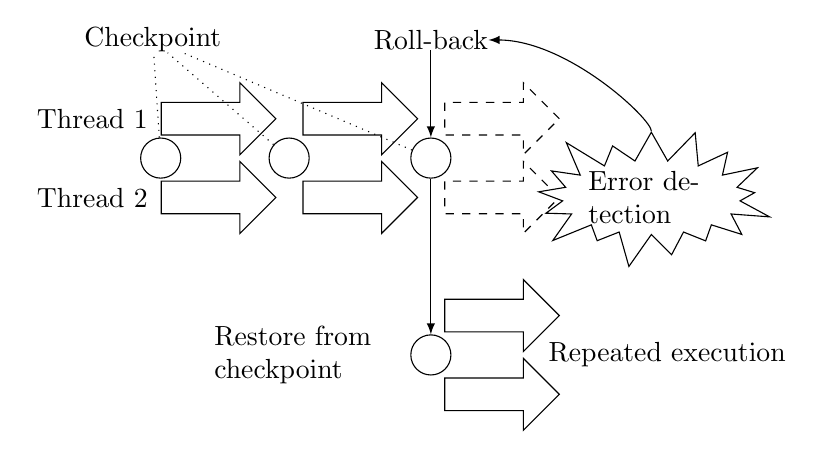
\begin{tikzpicture}[>=latex]
    \node (thread1) {Thread 1};
    \node[below of= thread1, node distance = 1cm] (thread2) {Thread 2};

    \node[draw, single arrow, node distance=1.5cm, inner ysep=0.2cm, text width = 1.cm, right of = thread1] (arrow11) {};
    \node[draw, single arrow, node distance = 1.8cm, inner ysep=0.2cm, text width = 1.cm, right of=arrow11] (arrow12) {};
    \node[dashed, draw, single arrow, node distance = 1.8cm, inner ysep=0.2cm, text width = 1.cm, right of=arrow12] (arrow13) {};

    \node[draw, single arrow, node distance=1.5cm, inner ysep=0.2cm, text width = 1.cm, right of = thread2] (arrow21) {};
    \node[draw, single arrow, node distance = 1.8cm, inner ysep=0.2cm, text width = 1.cm, right of=arrow21] (arrow22) {};
    \node[dashed, draw, single arrow, node distance = 1.8cm, inner ysep=0.2cm, text width = 1.cm, right of=arrow22] (arrow23) {};

    \node[fill=white, starburst, draw, right of = arrow23, node distance = 2.cm, text width = 1.6cm, inner sep = 0cm] (detection) {Error detection};

    \node[draw, circle, inner sep=0.18cm, at=(arrow11.west), yshift=-0.5cm] (chkpt0) {};
    \node[draw, circle, inner sep=0.18cm, right of=arrow11, yshift=-0.5cm] (chkpt1) {};
    \node[draw, circle, inner sep=0.18cm, right of=arrow12, yshift=-0.5cm] (chkpt2) {};
    \node[above of = chkpt2, node distance = 1.5cm, inner sep = 0cm] (rollback) {Roll-back};

    \node[above of= chkpt0, node distance=1.5cm, inner sep = 0cm, xshift=-0.1cm] (chkpts) {Checkpoint};
    \draw[dotted] (chkpt0) -- (chkpts);
    \draw[dotted] (chkpt1) -- (chkpts);
    \draw[dotted] (chkpt2) -- (chkpts);

    \node[draw, single arrow, node distance = 1.5cm, inner ysep=0.2cm, text width = 1.cm, below of=arrow23] (arrow33) {};
    \node[draw, single arrow, node distance = 1.cm, inner ysep=0.2cm, text width = 1.cm, below of=arrow33] (arrow43) {};
    \node[draw, circle, inner sep=0.18cm, below of=chkpt2, node distance=2.5cm] (chkpt2-restored) {};
    \node[left of = chkpt2-restored, node distance = 1.5cm, inner sep = 0cm, text width = 2.5cm] (restore) {Restore from checkpoint};

    \draw[->] (detection) .. controls +(0cm,1.cm) and +(1cm, 0cm).. (rollback.east);
    \draw[->] (rollback.south) .. controls +(0cm,-1cm) and +(0cm, 1cm).. (chkpt2.north);
    \draw[->] (chkpt2.south) .. controls +(0cm,-2cm) and +(0cm, 1cm).. (chkpt2-restored);

    \node[right of=chkpt2-restored, node distance = 3.cm] {Repeated execution};
  \end{tikzpicture}
\end{document}
